\chapter{Implementacija aplikacije LICC}
\label{chp:Implementation}

U ovom poglavlju će biti opisana implementacija pratećeg projekta nazvanog \emph{Language Invariant Code Comparer} (skr. \emph{LICC}), pisanog u programskom jeziku C\# 8.0, koristeći \emph{.NET Core 3.1} radni okvir. Lekseri i parseri za ulazne gramatike će u implementaciji takođe biti generisani u programskom jeziku C\#. C\# je izabran zbog lakoće implementacije velikih projekata i velike podrške paketa koji se mogu preuzeti, od kojih su korišćeni \emph{ANTLR Runtime} paket koji daje potrebne biblioteke za rad sa ANTLR generisanim parserima i \emph{Math.NET Symbolics} paket za rad sa simboličkim vrednostima. Rezultat je konzolna aplikacija koja može da generiše, serijalizuje ili prikaže opšti AST za dati izvorni k\^od, ali i da poredi takav AST sa drugim. Čitav projekat je dostupan u potpunosti na servisu GitHub na adresi \url{https://github.com/ivan-ristovic/LICC}.

Jedan od glavnih ciljeva aplikacije je modularnost i jednostavna proširivost. U tom duhu se, pored implementacije klasa potrebnih za predstavljanje opšte AST apstrakcije, pruža i interfejs za kreiranje adaptera koji će od proizvoljnog stabla parsiranja kreirati opšti AST. Kao primer, adapteri su kreirani za programske jezike C i Lua, a za primer potpune slobode u izboru gramatike je kreirana gramatika za pseudo-jezik i adapter za istu, što dozvoljava poređenje kodova sa specifikacijom datom u obliku pseudo-koda. Čitav projekat se sastoji od više komponenti, organizovanih po prostorima imena, od kojih su značajnije:
\begin{itemize}
    \item \texttt{LICC} --- Glavni program (korisnički interfejs) koji omogućava generisanje, prikaz, serijalizaciju i poređenje AST.
    \item \texttt{LICC.AST} ---Biblioteka klasa za rad sa opštom AST apstrakcijom.
    \item \texttt{LICC.Core} --- Upoređivač opštih AST --- konzolni izlaz.
    \item \texttt{LICC.Visualizer} --- Komponenta za vizualizaciju --- grafički prikaz AST.
    \item \texttt{LICC.Tests} --- Prateći testovi jedinica koda i integracioni testovi.
\end{itemize}

Čitava arhitektura data putem UML dijagrama komponenti se može videti na slici \ref{fig:ImplementationComponents}. Osim implementacije same aplikacije, svaki funkcionalni deo projekta prate i testovi jedinica koda, koji su povezani sa \emph{GitHub Actions} porškom za neprekidnu integraciju (engl. \emph{continuous integration}, srk. \emph{CI}). CI omogućava prevođenje izvornog koda nakon svake izmene kao i izvršavanje akcija nakon prevođenja kao što su testiranje ili generisanje predmeta za upotrebu (engl. \emph{artifacts}) koji predstavljaju rezultat procesa prevođenja i mogu se direktno isporučiti.

\begin{figure}[h!]
\centering
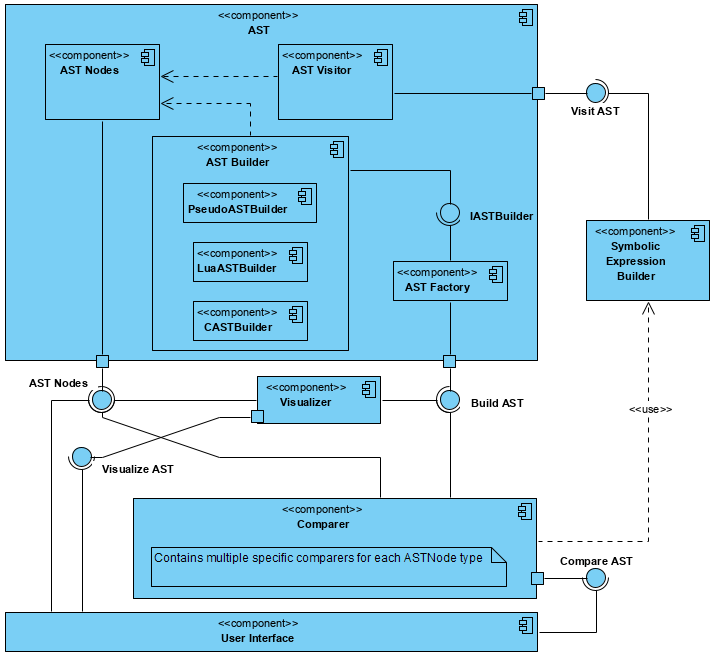
\includegraphics[scale=0.8]{images/uml/ComponentDiagram.png}
\caption{UML dijagram komponenti implementacije.}
\label{fig:ImplementationComponents}
\end{figure}


\section{Implementacija apstrakcije}
\label{sec:ImplementationMyAST}

Implementacija prati hijerarhije opisane u poglavlju \ref{chp:MyAST} kroz mehanizam nasleđivanja. Svaki tip čvora je implementiran kao zasebna klasa koja nasleđuje apstraktnu klasu \texttt{ASTNode}. Dijagram klasa koje nasleđuju klasu \texttt{ASTNode} se može videti na slikama \ref{fig:UMLASTNode1} i \ref{fig:UMLASTNode2}. Pored implementacije klasa koje predstavljaju AST čvorove, kreiran je i javno dostupni interfejs za obilazak AST putem obrazca posetilac u implementaciji korišćen za kreiranja graditelja simboličkog izraza od AST koji predstavlja izraz kao i evaluatora takvog AST.

\begin{figure}[h!]
\centering
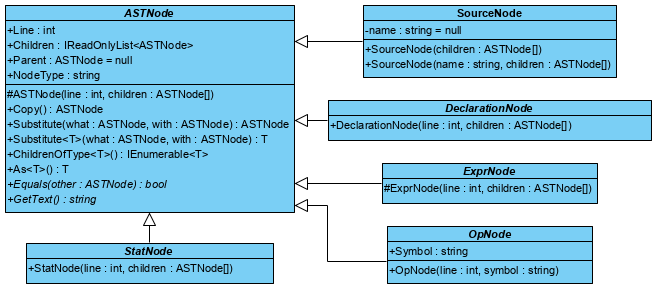
\includegraphics[scale=0.7]{images/uml/ASTNode.png}
\line(1,0){450}\\
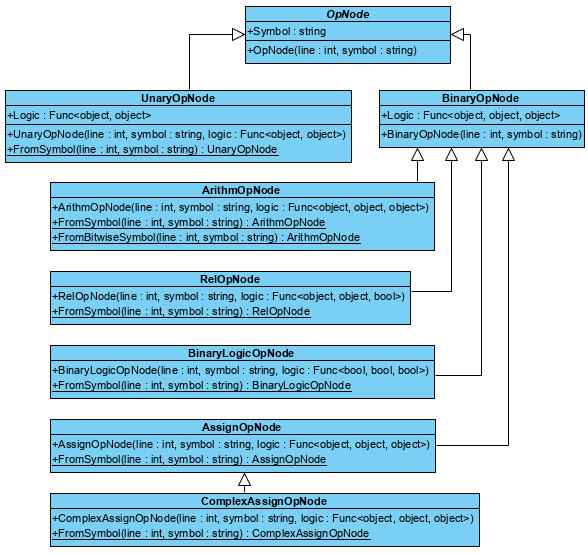
\includegraphics[scale=0.7]{images/uml/OperatorNode.png}
\caption{UML klasni dijagram (deo 1).}
\label{fig:UMLASTNode1}
\end{figure}

\begin{figure}[h!]
\centering
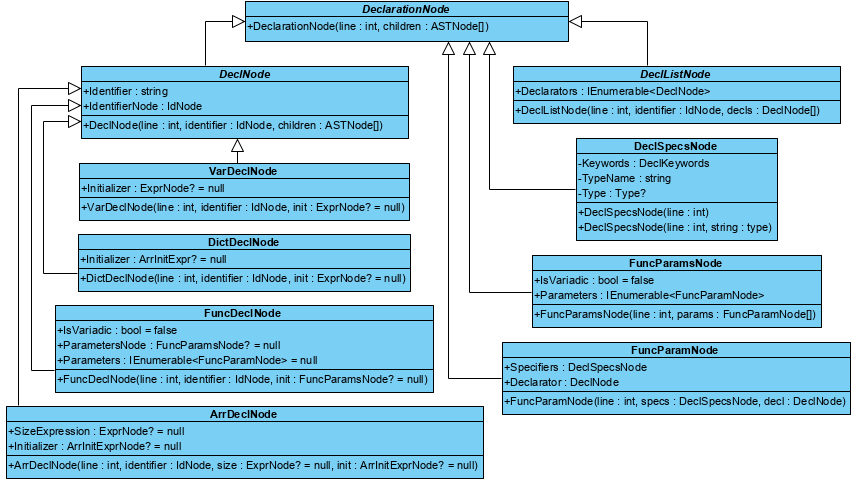
\includegraphics[scale=0.65]{images/uml/DeclarationNode.png}
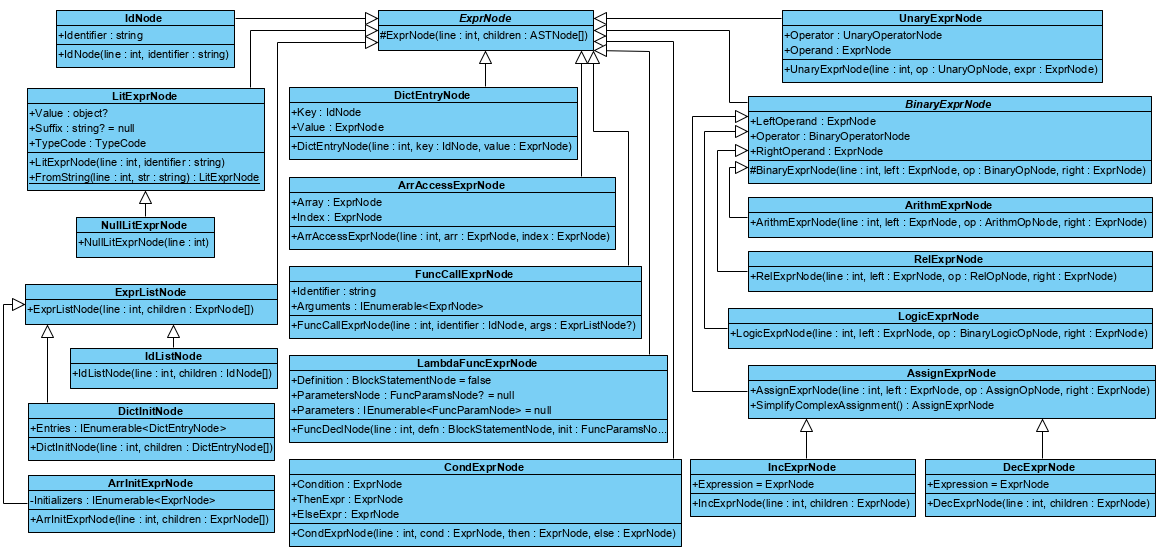
\includegraphics[scale=0.55]{images/uml/ExpressionNode.png}
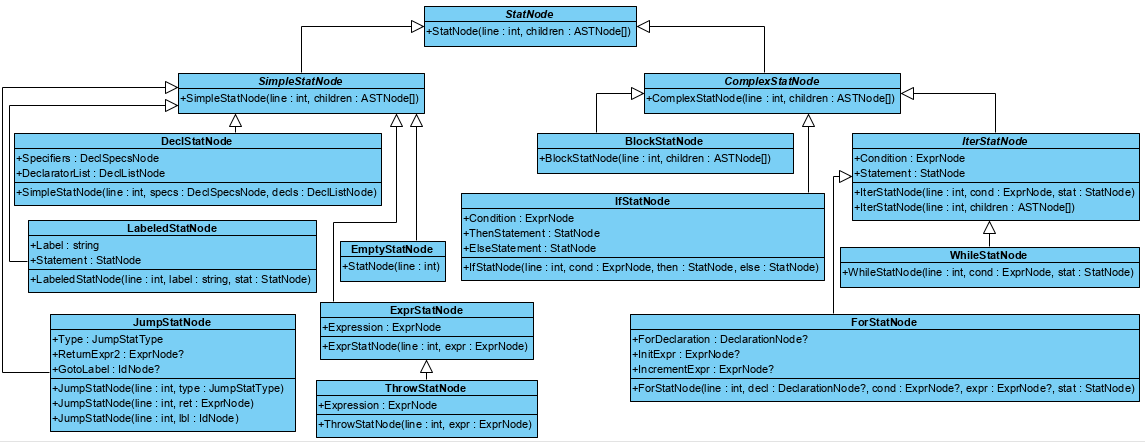
\includegraphics[scale=0.55]{images/uml/StatementNode.png}
\caption{UML klasni dijagram (deo 2).}
\label{fig:UMLASTNode2}
\end{figure}

AST struktura je \emph{imutabilna} --- ne mogu se dodavati ili uklanjati deca čvorovima. Moguće je klonirati AST čvorove ili vršiti zamenu određenog podstabla drugim podstablom ne menjajući original. Svaki AST čvor se može porediti po jednakosti sa drugim AST čvorom po intuitivnoj logici poređenja pruženom kroz predefinisane operatore poređenja.

\section{Implementacija upoređivača}
\label{sec:ImplementationComparer}

Implementacija algoritma upoređivača opisana u poglavlju \ref{chp:ASTComparing} se svodi na implementaciju funkcija za poređenje za svaki tip AST čvora. Te funkcije su enkapsulirane u klase koje implementiraju interfejs za upoređivač čvorova. Te klase nisu javne, tako da se poređenje vrši kroz upoređivač koji poredi instance tipa \texttt{ASTNode}, a koji putem refleksije određuje konkretni tip čvorova i, ukoliko su tipovi isti, pronalazi konkretni upoređivač i poziva operaciju interfejsa upoređivača. Upoređivači međusobno pozivaju jedni druge, kako bi se logika poređenja uprostila --- pošto se naredbe deklaracije sastoje od specifikatora deklaracije i liste deklaratora, upoređivač naredbi deklaracije može pozivati upoređivač za specifikatore deklaracije i upoređivač za listu deklaratora. 

Upoređivač kao rezultat svog rada vraća kolekciju potencijalnih problema (upozorenja ili grešaka) koje je detektovao prilikom analize. Ovakav pristup je odabran zbog lakoće testiranja upoređivača, s obzirom da se može očekivati određena kolekcija problema za određeni izvorni kod. Problem se modeluje kao apstraktna klasa \texttt{BaseIssue} dok se upozorenja ili greške modeluju kroz njene konkretizacije \texttt{BaseWarning} i \texttt{BaseError}. Konkretne greške, kao što su npr. nedostatak deklaracija se mogu onda modelovati kao konkretizacije ovih klasa u zavisnosti od ozbiljnosti problema. Primer izlaza upoređivača za algoritam \emph{swap} se može videti na slici \ref{fig:ComparerSwap}.

\begin{figure}[h!]
\centering
%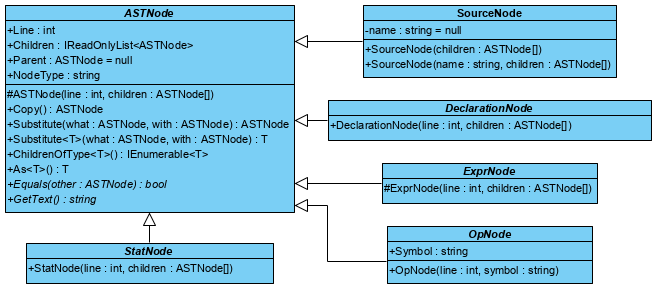
\includegraphics[scale=0.7]{images/uml/ASTNode.png}
\caption{Rezultat rada upoređivača za \texttt{swap} algoritam.}
\label{fig:ComparerSwap}
\end{figure}

\section{Implementacija vizualnog prikaza AST}
\label{sec:ImplementationVisualizer}

Osim serijalizacije AST u JSON format, kreiran je potprogram za vizualni prikaz AST-a (u daljem tekstu \emph{vizualizator}). Primeri izlaza vizualizatora se mogu videti na slikama iz poglavlja \ref{chp:MyAST} --- \ref{fig:MyASTExampleCDeclaration}, \ref{fig:MyASTExampleLuaDeclaration}, \ref{fig:MyASTExampleExpressions} i \ref{fig:MyASTExampleStatement}. Prikaz je izvršen koristeći nativni \texttt{Graphics} paket i, s obzirom da je u pitanju \emph{.NET Core 3.1} radni okvir, moguće je dobiti vizualni prikaz nezavisno od sistema.

Vizualizacija počiva na rekurzivnom algoritmu prikaza u dubinu --- za svaki čvor se prikažu potomci, rasporede jednako po širini, a onda se roditelj centrira u odnosu na ukupnu širinu koju zauzimaju deca. Ovaj pristup nije prostorno optimalan, zbog varijacija u broju dece za čvorove različitih tipova. Što se informacija za svaki čvor tiče, prikazuju se vrednosti svih atributa čvora zajedno sa njegovim tipom u zaglavlju kao i grane do njegovih potomaka.

\section{Implementacija korisničkog interfejsa}
\label{sec:ImplementationUI}

S obzirom da je aplikacija konzolna (osim komponente za vizualizaciju), korisnički interfejs se svodi na argumente komandne linije. Pokretanje programa bez argumenata pruža prikaz za pomoć u kome su nabrojane sve opcije, prikazano na slici \ref{fig:UIImpl}.

\begin{figure}[h!]
\centering
%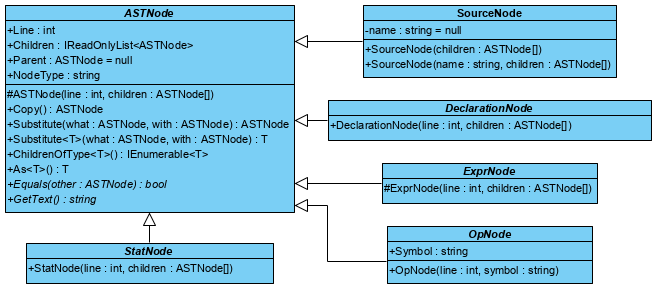
\includegraphics[scale=0.7]{images/uml/ASTNode.png}
\caption{Korisniči interfejs programa pružen kroz argumente komandne linije.}
\label{fig:UIImpl}
\end{figure}

\section{Testovi}
\label{sec:ImplementationTests}

Komponentu za kreiranje AST i komponentu za poređenje AST prate testovi jedinica koda. Testovi su organizovani u zasebnom projektu na sledeći način:
\begin{itemize}
    \item \texttt{LICC.Tests.AST} --- Testovi za adaptere i posetioce, kao i testovi funkcionalnosti metoda klase \texttt{ASTNode}.
    \item \texttt{LICC.Tests.Core} --- Testovi upoređivača.
\end{itemize}

Radni okvir koji se koristi za testiranje je \texttt{NUnit}\footnote{\url{https://nunit.org/}} koji pruža tzv. \emph{model ograničenja} (engl. \emph{constraint model}) i time omogućava pisanje čitljivog koda. Pisanje testova po modelu ograničenja se sastoji od korišćenja jednog metoda za pisanje svih testova koji kao argumente prima objekat koji se testira i složeni objekat koji predstavlja ograničenje koje objekat koji se testira treba da zadovoljava. Primer testa pisanog u ovom radnom okviru uz model ograničenja u kontekstu implementacije ovog rada se može videti na slici \ref{fig:ImplTestsUnit}.

\begin{figure}[h!]
\centering
\begin{lstlisting}
[Test]
public void ComplexDefinitionTest()
{
    FuncDefNode f = this.AssertFunctionSignature(@"
        float f(const unsigned int x, ...) {
            int z = 4;
            return 3.0;
        }", 
        2, "f", "float", isVariadic: true, 
        @params: ("unsigned int", "x")
    );
    Assert.That(f.IsVariadic);
    Assert.That(f.Definition.Children, Has.Exactly(2).Items);
}

protected FuncDefNode AssertFunctionSignature(
    string src, int line, string fname, 
    string returnType = "void", bool isVariadic = false, 
    AccessModifiers access = AccessModifiers.Unspecified,
    QualifierFlags qualifiers = QualifierFlags.None, 
    params (string Type, string Identifier)[] @params)
{
    FuncDefNode f = this.GenerateAST(src).As<FuncDefNode>();
    this.AssertChildrenParentProperties(f);
    this.AssertChildrenParentProperties(f.Definition);
    Assert.That(f, Is.Not.Null);
    Assert.That(f.Line, Is.EqualTo(line));
    Assert.That(f.Declarator, Is.Not.Null);
    Assert.That(f.Declarator.Parent, Is.EqualTo(f));
    Assert.That(f.Keywords.AccessModifiers, Is.EqualTo(access));
    Assert.That(f.Keywords.QualifierFlags, Is.EqualTo(qualifiers));
    Assert.That(f.Identifier, Is.EqualTo(fname));
    Assert.That(f.ReturnTypeName, Is.EqualTo(returnType));
    Assert.That(f.IsVariadic, Is.EqualTo(isVariadic));
    if (@params?.Any() ?? false) {
        Assert.That(f.Parameters, Is.Not.Null);
        Assert.That(f.Parameters, Has.Exactly(@params.Length).Items);
        Assert.That(f.ParametersNode, Is.Not.Null);
        Assert.That(
            f.Parameters.Select(
                p => (p.Specifiers.TypeName, p.Declarator.Identifier)
            ), 
            Is.EqualTo(@params)
        );
    }
    return f;
}
\end{lstlisting}
\caption{Primer jediničnog testa za proveru generisanog AST čvora za datu funkciju.}
\label{fig:ImplTestsUnit}
\end{figure}

Osim testova jedinica koda, prisutni su i testovi integracije svih komponenti. Kao što je opisano u prethodnim odeljcima, rezultat rada adaptera je AST, dok je rezultat data upoređivača za data dva stabla kolekcija problema. Ta dva odvojena procesa se onda mogu spojiti kako bi se testirala integracija te dve komponente --- dakle, od dva programa očekivati određenu kolekciju problema. Primer za \emph{swap} algoritam se može videti na slici \ref{fig:ImplTestsIntegration}.

\begin{figure}[h!]
\centering
\begin{lstlisting}
[Test]
public override void DifferenceTests()
{
    this.Compare(
        this.FromPseudoSource(@"
            algorithm Swap 
            begin
                declare integer x = vx
                declare integer y = vy
                procedure swap()
                begin
                    declare integer tmp = x
                    x = y  
                    y = tmp
                end
            end
        "),
        this.FromCSource(@"
            int x = vx, y = vy;
            void swap() {
                int tmp = x; y = tmp; x = y;
            }
        "),
        new MatchIssues()
            .AddError(
                new BlockEndValueMismatchError("x", 1, "vy", "vx")
            )
            .AddError(
                new BlockEndValueMismatchError("x", 3, "vy", "vx")
            )
    );
}

protected void Compare(ASTNode src, ASTNode dst, 
    MatchIssues? expectedIssues = null)
{
    expectedIssues ??= new MatchIssues();
    MatchIssues issues = new ASTNodeComparer(src, dst)
        .AttemptMatch();
    Assert.That(issues, Is.EquivallentTo(expectedIssues));
}
\end{lstlisting}
\caption{Primer kompletnog testa za algoritam \emph{swap}.}
\label{fig:ImplTestsIntegration}
\end{figure}

\section{Primeri upotrebe LICC}
\label{sec:ImplementationExample}

U ovom odeljku će biti prikazano par slučajeva upotrebe implementirane aplikacije. Prvo će biti pokazan primer generisanja opšteg AST u JSON formatu a zatim i primer poređenje dve implementacije istog algoritma u dva različita programska jezika. Algoritam koji će biti korišćen u nastavku kao primer je algoritam zamene vrednosti promenljivih implementiran kroz funkciju \texttt{swap} koja menja vrednosti dveju globalnih promenljivih. Na slici \ref{fig:ExampleSwap} se mogu videti implementacije ovog algoritma koje će biti polazne tačke za kreiranje opšteg AST i poređenja istih.

\begin{figure}[h!]
\begin{lstlisting}
int x = vx, y = vy;

void swap() 
{
    int tmp = y;
    y = x;
    x = tmp;
}
\end{lstlisting}
\begin{lstlisting}
x = vx
y = vy
function swap()
	x, y = y, x
end
\end{lstlisting}
\begin{lstlisting}
algorithm Swap 
begin
    declare integer x = vx
    declare integer y = vy
    procedure swap()
    begin
        declare integer tmp 
        tmp = x
        x = y  
        y = tmp
    end
end
\end{lstlisting}
\caption{Izvorni kodovi algoritma \texttt{swap} u programskim jezicima C (gore), Lua (sredina) i u pseudojeziku (dole).}
\label{fig:ExampleSwap}
\end{figure}


\subsection{Generisanje opšteg AST}
\label{subsec:ImplementationExampleAST}

AST je moguće generisati od izvornog koda navođenjem glagola \texttt{ast}. Ukoliko su na fajl sistemu dostupni izvorni kodovi sa sadržajima sa slike \ref{fig:ExampleSwap}, moguće je generisati opšti AST u JSON formatu zadavanjem glagola \texttt{ast} kao na slici \ref{fig:ExampleSwapAST}. U gornjem delu slike je prikazan samo deo izlaza zbog veličine generisanog JSON sadržaja), u srednjem delu slike je prikazan kompaktni JSON ispis zadat opcijom \texttt{-c}, dok je u donjem delu slike prikazan ispis zadat opcijom \texttt{-v} pri čemu je prikazan samo dao izlaza koji se generiše prilikom posećivanja stabla parsiranja i generisanja AST čvorova.

\begin{figure}[h!]
\centering
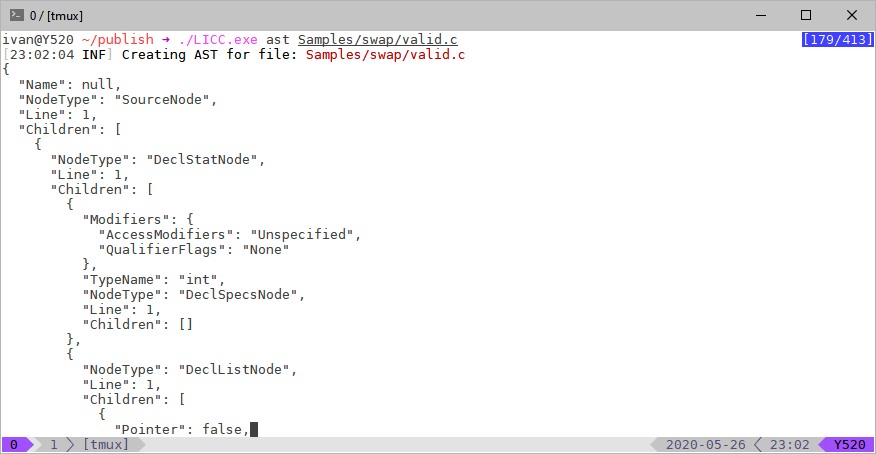
\includegraphics[scale=0.6]{images/eval/ast_c.png}
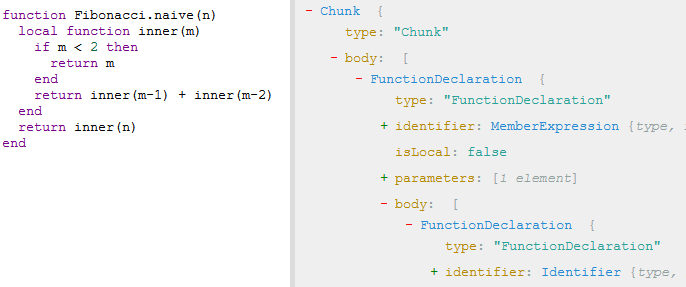
\includegraphics[scale=0.6]{images/eval/ast_lua.png}
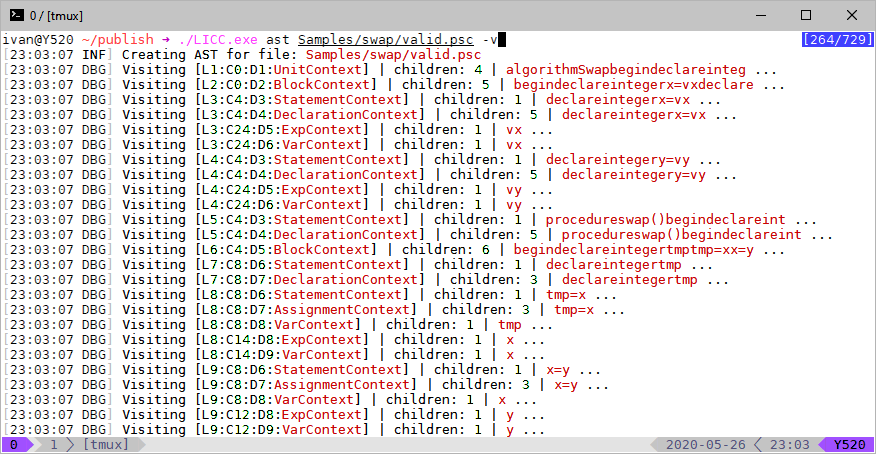
\includegraphics[scale=0.6]{images/eval/ast_psc.png}
\caption{Vizualni prikaz generisanja AST od izvornih kodova sa slike \ref{fig:ExampleSwap} redom.}
\label{fig:ExampleSwapAST}
\end{figure}


\subsection{Poređenje opštih AST}
\label{subsec:ImplementationExampleComparer}

Jedan od osnovnih slučajeva upotrebe alata LICC može biti testiranje validnosti implementacije na osnovu date specifikacije. Ukoliko kao specifikaciju za algoritam \texttt{swap} uzmemo izvorni kod u pseudo-jeziku, možemo testirati da li su implementacije u programskim jezicima C ili Lua semantički ekvivalentne specifikaciji. Izlaz rada LICC za verifikaciju implementacije algoritma \texttt{swap} u programskom jeziku Lua u odnosu na specifikaciju u pseudo-jeziku se može videti na slici \ref{fig:ExampleSwapCompareValid}. Primetimo da su prisutna upozorenja o odudaranju tipova --- Lua nije striktno tipiziran jezik, a specifikacija nalaže da su globalne promenljive celi brojevi, dok su u implementaciji one tipa \texttt{object}, što može biti potencijalni problem ali s obzirom na prirodu skript jezika nije prijavljeno kao greška.

\begin{figure}[h!]
\centering
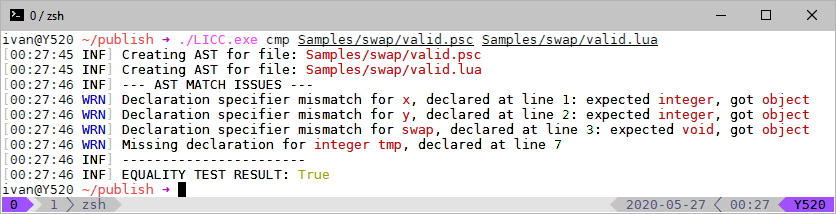
\includegraphics[scale=0.65]{images/eval/cmp_valid.png}
\caption{Semantičko poređenje implementacija sa slike \ref{fig:ExampleSwap} (Lua u odnosu na pseudo-jezik).}
\label{fig:ExampleSwapCompareValid}
\end{figure}

Ukoliko pak izvorni kod ne odgovara specifikaciji, LICC će dati detaljan spisak razlika, koje su često tražene greške. U nekim slučajevima je moguće da je sematnička ekvivalentnost održana iako stabla imaju značajne razlike --- LICC će prijaviti sve te razlike kao greške iako one to možda nisu. Izlaz za poređenje nevalidne implementacije algoritma \texttt{swap} sa slike \ref{fig:ExampleSwapWrong} u odnosu na specifikaciju se može videti na slici \ref{fig:ExampleSwapCompareWrong}. Vidimo da jedna od globalnih promenljivih nije pravilno zamenila vrednost, što se detektuje dvaput --- po jednom za svaki od blokova u izvornom kodu. Dodatno, prijavljena je i greška o odudaranju izraza inicijalizatora za promenljivu \texttt{tmp}.

\begin{figure}[h!]
\begin{lstlisting}
int x = vx, y = vy;

void swap() {
    int tmp = x;
    y = tmp;
    x = y;
}
\end{lstlisting}
\caption{Nevalidna implementacija algoritma \texttt{swap} (C).}
\label{fig:ExampleSwapWrong}
\end{figure}

\begin{figure}[h!]
\centering
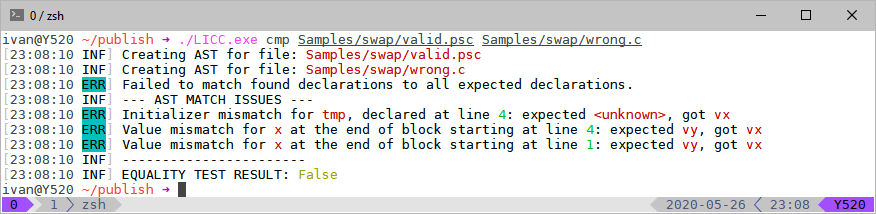
\includegraphics[scale=0.65]{images/eval/cmp_wrong.png}
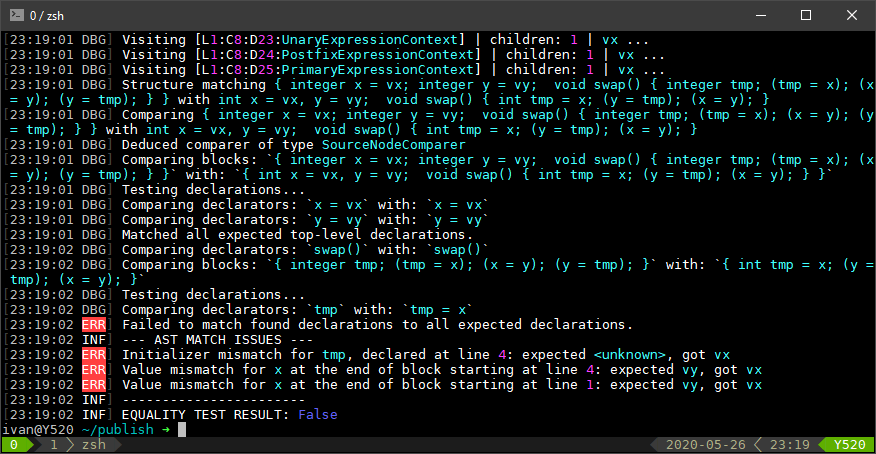
\includegraphics[scale=0.65]{images/eval/cmp_wrong_v.png}
\caption{Semantičko poređenje nevalidne implementacije sa slike \ref{fig:ExampleSwapWrong} u odnosu na specifikaciju sa slike \ref{fig:ExampleSwap}.}
\label{fig:ExampleSwapCompareWrong}
\end{figure}

Ukoliko imamo već verifikovanu implementaciju algoritma u jednom programskom jeziku, može se desiti potreba za prelaskom na novije tehnologije što uključuje i prepisivanje algoritma sa jednog programskog jezika na drugi. LICC se može iskoristiti za poređenje tih implementacija, konkretno za algoritam \texttt{swap} na slici \ref{fig:ExampleSwapCompareValidRewrite} se može videti rezultat poređenja implementacija u programskim jezicima C i Lua, pri čemu je takođe prikazan izlaz koji se dobija ukoliko se navede opcija \texttt{-v}. 

\begin{figure}[h!]
\centering
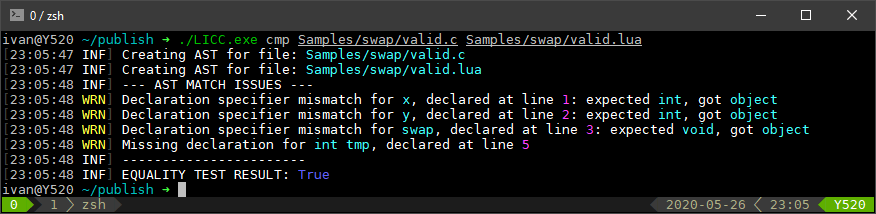
\includegraphics[scale=0.7]{images/eval/cmp_rewrite.png}
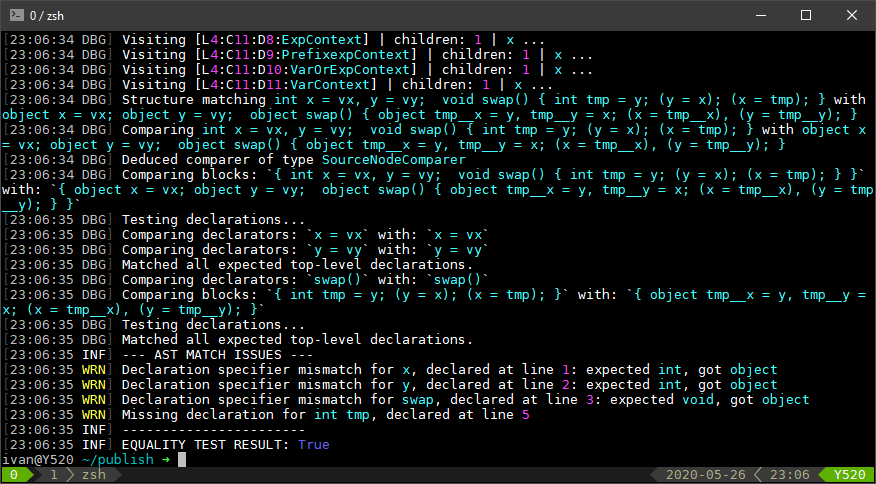
\includegraphics[scale=0.7]{images/eval/cmp_rewrite_v.png}
\caption{Semantičko poređenje implementacija sa slike \ref{fig:ExampleSwap}.}
\label{fig:ExampleSwapCompareValidRewrite}
\end{figure}

Još jedan slučaj upotrebe LICC može biti verifikacija međuverzija koda u procesu refaktorisanja. LICC pretpostavlja strukturnu sličnost kodova, što u procesu refaktorisanja često implicitno važi, ili barem važi u malim koracima između polazne i finalne verzije nakon refaktorisanja. Ukoliko refaktorišemo implementaciju algoritma \texttt{swap} u programskom jeziku C i dobijemo izvorni kod sa slike \ref{fig:ExampleSwapRefactor}, možemo uporediti tu implementaciju sa već verifikovanom implementacijom u programskom jeziku C. Rezultat rada upoređivača se može videti na slici \ref{fig:ExampleSwapCompareRefactor} --- primećujemo da je jedino detektovano da nedostaje promenljiva \texttt{tmp}, vrednosti globalnih promenljivih su iste u odnosu na specifikaciju na kraju svakog od blokova.

\begin{figure}[h!]
\begin{lstlisting}
int x = vx, y = vy;

void swap() 
{
    x = x + y;
	y = x - y;
	x = x - y;
}
\end{lstlisting}
\caption{Refaktorisani algoritam \texttt{swap} (C).}
\label{fig:ExampleSwapRefactor}
\end{figure}

\begin{figure}[h!]
\centering
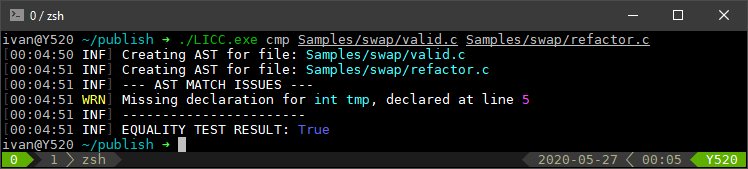
\includegraphics[scale=0.8]{images/eval/cmp_refactor.png}
\caption{Semantičko poređenje refaktorisane implementacije algoritma \texttt{swap} sa slike \ref{fig:ExampleSwapRefactor} sa implementacijom u programskom jeziku C sa slike \ref{fig:ExampleSwap}.}
\label{fig:ExampleSwapCompareRefactor}
\end{figure}

